\documentclass[acmtog, authorversion, acmlarge]{acmart}
\usepackage{enumitem}
\usepackage{listings}
\usepackage{amsmath, amsthm}
\usepackage{stmaryrd}
\usepackage{proof} 
\usepackage{semantic}
\usepackage{xifthen}
\usepackage{subcaption}
\usepackage{wrapfig}
\usepackage{IEEEtrantools}


% Tell latex I really dislike it when you break my inline math!
\relpenalty=10000
\binoppenalty=10000

% I am a simple proof kinda guy
\newtheorem{thm}{Theorem}
\newtheorem{lem}{Lemma}
\newtheorem{cor}{Corollary}
\newtheorem{pos}{Postulate}
% Metadata Information
%% \acmJournal{TOG}
%% \acmVolume{9}
%% \acmNumber{4}
%% \acmArticle{39}
%% \acmYear{2010}
%% \acmMonth{3}

% Copyright
%\setcopyright{none}
%\setcopyright{acmlicensed}
\setcopyright{rightsretained}
%\setcopyright{usgov}
%\setcopyright{usgovmixed}
%\setcopyright{cagov}
%\setcopyright{cagovmixed}

% DOI
\acmDOI{}

% Paper history
%\received{February 2007}
%\received{March 2009}
%\received[final version]{June 2009}
%\received[accepted]{July 2009}


% Document starts
\begin{document}
% Title portion
\title{Hyper-Coercions}
\author{Andre Kuhlenschmidt}
\affiliation{%
  \institution{Indiana University}
}

\renewcommand\shortauthors{A. Kuhlenschmidt}

\begin{abstract}
\end{abstract}

\maketitle

%% Types
%% the type meta variable

\newcommand{\T}{\ensuremath{T}}
\newcommand{\B}{\ensuremath{B}}
\newcommand{\I}{\ensuremath{I}}
\newcommand{\Fn}[3][]{\ensuremath{#2 #1 \to #1 #3}}
\newcommand{\Ref}[1]{\ensuremath{\texttt{Ref} \, #1}}
\newcommand{\Integer}{\ensuremath{\texttt{Int}}}
\newcommand{\Bool}{\ensuremath{\texttt{Bool}}}
\newcommand{\Dyn}{\ensuremath{\star}}


%% Blame labels
\newcommand{\Lbl}{\ensuremath{\ell}}

%% Hyper Coercion Syntax
\newcommand{\Prj}{\ensuremath{p}}
\newcommand{\pmt}{\ensuremath{\id}}
\newcommand{\Med}{\ensuremath{\mu}}
\newcommand{\Inj}{\ensuremath{i}}
\newcommand{\imt}{\ensuremath{\pmt}}
\newcommand{\HC}{\ensuremath{h}}
\newcommand{\hc}[5]{\ensuremath{\, #1 #2 #3 #4 #5 \,}}
\newcommand{\hcfail}[5]{\ensuremath{#1 #2 \failed{#3}{#4}{#5}}}

% Hyper-Coercion Syntax Shared with Coercions
\newcommand{\prj}[2][]{\ensuremath{#1 ?^{#2}}}
\newcommand{\inj}[1][]{\ensuremath{#1 !}}
\newcommand{\failed}[3]{\ensuremath{\bot^{#1 #2 #3}}}
\newcommand{\id}[1][]{\ensuremath{\iota_{#1}}}
\newcommand{\fn}[3][]{\ensuremath{#2 #1 \to #1 #3}}
\newcommand{\rf}[2]{\ensuremath{\texttt{Ref} \, #1 \, #2}} 

% Coercions Syntax
\newcommand{\Crcn}{\ensuremath{c}}
\newcommand{\SE}{\ensuremath{s}}
\newcommand{\Int}{\ensuremath{m}}
\newcommand{\Fnl}{\ensuremath{f}}
\newcommand{\Seq}[2]{\ensuremath{#1 ; #2}}

%% Consistency, Shallow Consistency, and Shallow Inconsistency
\newcommand{\sct}[1][\;]{\ensuremath{#1 \overline{\#} #1}}
\newcommand{\sic}[1][\;]{\ensuremath{#1 \# #1}}

%% Hyper Coercion and Coercion Well Typed Judgment
\newcommand{\cwt}[3]{\ensuremath{\vdash \, #1 \, : \, #2 \Rightarrow #3}}

%% Cast and Make Coercion Relation
\newcommand{\cast}[3][\Lbl]{\ensuremath{#2 \Rightarrow^{#1} #3}}
\newcommand{\mkcrcn}[3][\Lbl]{\ensuremath{\langle \cast[#1]{#2}{#3} \rangle}}
\newcommand{\mkIcrcn}[3][\Lbl]{\ensuremath{\{ \cast[#1]{#2}{#3} \}}}
\newcommand{\mkmed}[3][\Lbl]{\ensuremath{\langle \widehat{\cast[#1]{#2}{#3}} \rangle}}

%% Compose and Compose Mediating Coercions
\newcommand{\cmp}[2]{\ensuremath{#1 \fatsemi #2}}
\newcommand{\cmpm}[2]{\cmp{#1}{#2}}

%% Metafunctions
\newcommand{\depth}[1]{\ensuremath{\mid #1 \mid}}
\newcommand{\Max}[1]{\ensuremath{\texttt{max}(#1)}}

%% Compiling to / from
\newcommand{\interp}[3]{%
  \ensuremath{\llbracket #1 \rrbracket_{#3}^{#2}}}

\newcommand{\interpm}[3]{%
  \ensuremath{\llbracket \overline{#1} \rrbracket_{#3}^{#2}}}


\section{Syntax, Typing, and Composition}
\label{sec:hc}

Hyper-Coercions are a densely packed version of space-efficient
coercions in the style of \citet{Siek:2015ab} which we hope to use to
increase the performance of gradually typed programs. 
%
The main intuition behind their formulation is that the longest
sequence of coercions in \citet{Siek:2015ab} is a series of a
projection, then cast intermediating between two possibly equal types,
followed a injection; the hyper-coercion structure can represent this
longest chain of coercions in a single hyper-coercion node.
%
When we translate model to the implementation this means that a direct
implementation should have to follow less pointers because the
representation keep all subcomponent in the same structure.
%
A hyper-coercion (\HC \; in
Figure~\ref{fig:hcSyntax}) is a 5-tuple that contain a projection
(\Prj), the source type and target types (\T{}s) of the intermediating
coercion (\Med), the intermediating coercion itself, and finally an
injection (\Inj). Figure~\ref{fig:hcTyping} shows the typing judgments
for hyper-coercions and their subcomponent coercions.  We can seen
that a hyper-coercion, \hc{\Prj}{\T_2}{\Med}{\T_3}{\Inj}, is
well-typed cast from $\T_1$ to $\T_2$ if there is well-typed
projection (\Prj) from $\T_1$ to $\T_2$, a well-typed intermediating
cast (\Med) from $\T_2$ to $\T_3$, and well typed injection from
$\T_2$ to $\T_3$.

If a previous composition operation (shown in
Figure~\ref{fig:hcCompose}) resulted in a failed coercion then the
alternative \emph{failed hyper-coercion}
(\hcfail{\Prj}{\I}{\I_{2}}{\Lbl}{\I_{3}}) is used to signify that
after a projection (\Prj) to type (\T), the failed hyper-coercion will
report an error due to inconsistency between injectable (non-dynamic)
types $\I_1$ and $\I_2$. This failure will blame $\Lbl$ if it is applied,
but the projection must be preserved because it also has the
potential to fail before
this error is reported. A failed coercion is well-typed from $\T_1$ to
$\T_2$ if the projection is well-typed from $\T_1$ to $\I_1$, $\I_1$
is shallow consistent with $\I_2$, and $I_2$ is shallow inconsistent
with $\I_3$.

The rest of typing judgments are standard. Syntactically, projections
and injections differ in that they no longer contain the types that they
project to and inject from. Instead their source and target types
are shared with the overall hyper-coercion. This is merely to reduce
the complexity of composition rules and reflects the mindset of
considering a sequence of casts as a single entity.

The compose operation on hyper-coercions is a direct translation
of the compose operation of \citet{Siek:2015ab}. The larger granularity
of hyper-coercions causes a need for some special cases when
handling failure, but we have found a way around this in our
actual implementation which we discussed in Section~\ref{sec:schml}.

We have formalized this model in Coq and proven that compose preserves
the well-typing of hyper-coercions, that hyper-coercions are
isomorphic to space-efficient coercions, and that this isomorphism
respects the composition operation. Sections~\ref{sec:well-typing}
and~\ref{sec:iso} explain these proofs. Section~\ref{sec:schml}
discusses how the implementation differs from the model shown in
Figure~\ref{fig:hc}, and Section~\ref{sec:perf} presents benchmark
results that indicate the initial implementation does not improve the
performance over our current coercions implementation.


\begin{figure}[tbh]
  \small
  \begin{subfigure}{.5\textwidth}
    \[
    \begin{array}{llcl}
      \textbf{Base Types} &
      \B & := & \Integer \mid \Bool \\
      \textbf{Types} &
      \T    & ::= & \B \mid \Fn{\T}{\T} \mid \Ref{\T} \mid \Dyn \\
      \textbf{Injectable Types} &
      \I    & ::= & \B \mid \Fn{\T}{\T} \mid \Ref{\T} \\
      \textbf{Projections}&
      \Prj  & ::= & \pmt \mid \prj{\Lbl} \\
      \textbf{Injections}&
      \Inj  & ::= & \imt \mid \; \inj \\
      \textbf{Intermediates}&
      \Med  & ::= & \id \mid \fn{\HC}{\HC} \mid \rf{\HC}{\HC}\\
      \textbf{Hyper Coercions}&
      \HC   & ::= & \hc{\Prj}{\T}{\Med}{\T}{\Inj} \mid \hcfail{\Prj}{\T}{\I}{\Lbl}{\I}
    \end{array}
    \]
    \caption{Syntax of Hyper Coercions}
    \label{fig:hcSyntax}
  \end{subfigure}%
  \begin{subfigure}{0.5\textwidth}
    \begin{gather*}
      \inference{}{\B \sct \B}
      \quad
      \inference{}{\Fn{\T_{11}}{\T_{12}} \sct \Fn{\T_{21}}{\T_{22}}}
      \\[2ex]
      \inference{}{\Ref{\T_{1}} \sct \Ref{\T_{2}}}
      \quad
      \inference{}{\Dyn \sct \T}
      \quad
      \inference{}{\T \sct \Dyn}
      \\[2ex]
      \inference{\neg (\T_1 \sct \T_2)}{\T_1 \sic \T_2}
    \end{gather*}
    \caption{Shallow Consistency(\sct) and Inconsistency (\sic)}
    \label{fig:shallowConsistency}
  \end{subfigure}
  \begin{subfigure}{.5\textwidth}
    \begin{gather*}
      %% \inference{}{\cwt{\pmt}{\T}{\T}}
      %% \\[2ex]
      \inference{}{\cwt{\prj{\Lbl}}{\Dyn}{\I}}
      \quad
      \inference{\cwt{\HC_1}{\T_{3}}{\T_{1}} &
                 \cwt{\HC_2}{\T_{2}}{\T_{4}}}
                {\cwt{\fn{\HC_1}{\HC_2}}
                     {\Fn{\T_{1}}{\T_{2}}}
                     {\Fn{\T_{3}}{\T_{4}}}}
      \\[2ex]
      \inference{}{\cwt{\inj}{\I}{\Dyn}}      
      \quad
      \inference{\cwt{\HC_1}{\T_{2}}{\T_{1}} &
                 \cwt{\HC_2}{\T_{1}}{\T_{2}}}
                {\cwt{\rf{\HC_1}{\HC_2}}
                     {\Ref{\T_{1}}}
                     {\Ref{\T_{2}}}}
      \\[2ex]
      \inference{}{\cwt{\id}{\T}{\T}}
      \quad          
      \inference{\cwt{\Prj}{\T_1}{\I_1} &
                 \I_1 \sct \I_2 &
                 \I_2 \sic \I_3}
                {\cwt{\hcfail{\Prj}{\I_1}{\I_2}{\Lbl}{\I_3}}{\T_1}{\T_2}}
      \\[2ex]
      \inference{\cwt{\Prj}{\T_1}{\T_2} &
                 \cwt{\Med}{\T_2}{\T_3} &
                 \cwt{\Inj}{\T_3}{\T_4}}
                {\cwt{\hc{\Prj}{\T_2}{\Med}{\T_3}{\Inj}}{\T_1}{\T_4}}
    \end{gather*}
    \caption{Typing Judgment}
    \label{fig:hcTyping}
  \end{subfigure}%
  \begin{subfigure}{.5\textwidth}
    \begin{align*}
      \mkcrcn{\T}{\T} &= \hc{\pmt}{\T}{\id}{\T}{\imt} \\
      %
      \mkcrcn{\Dyn}{\I} &= \; \hc{\prj{\Lbl}}{\I}{\id}{\I}{\imt} \\
      %
      \mkcrcn{\I}{\Dyn} &= \hc{\pmt}{\I}{\id}{\I}{\inj} \\
      %
      \mkcrcn{\Fn[\!]{\T_{1}}{\T_{2}}}{\Fn[\!]{\T_{3}}{\T_{4}}} &=
         \hc{\pmt}{\Fn[\!]{\T_{1}}{\T_{2}}}
            {(\fn[\!]{\mkcrcn{\T_{3}}{\T_{1}}}{\mkcrcn{\T_{2}}{\T_{4}}})} 
            {\Fn[\!]{\T_{3}}{\T_{4}}}{\imt} \\ 
            & \hspace{5.3em} \texttt{if} \; % 
            \Fn[\!]{\T_{1}}{\T_{2}} \neq \Fn[\!]{\T_{3}}{\T_{4}} \\
      %
      \mkcrcn{\Ref{\T_1}}{\Ref{\T_2}} &=
         \hc{\pmt}{\Ref{\T_{1}}}
            {(\rf{\mkcrcn{\T_{2}}{\T_{1}}}{\mkcrcn{\T_{1}}{\T_{2}}})} 
            {\Ref{\T_{2}}}{\imt} \\
            & \hspace{5.3em} \texttt{if} \; % 
            \Ref{\T_1} \neq \Ref{\T_2} \\
      %
      \mkcrcn{\I_1}{\I_2} &= \hcfail{\pmt}{\I_1}{\I_1}{\Lbl}{\I_2} %
      \hspace{.6em} \texttt{if} \; \I_1 \sic \I_2
    \end{align*}
    \caption{Make Hyper-Coercion}
    \label{fig:hcMakeCoercion}
  \end{subfigure}
  \begin{subfigure}{.5\textwidth}
    \begin{align*}
      %
      \cmp{\hc{\pmt}{\Dyn}{\id}{\Dyn}{\imt}}{\HC} &= \HC \\
      %
      \cmp{\hc{\Prj}{\I_1}{\Med}{\I_2}{\inj}} %
          {\hc{\pmt}{\Dyn}{\id}{\Dyn}{\imt}} %
      &=  \hc{\Prj}{\I_1}{\Med}{\I_2}{\inj} \\
      % Comp_hc_no_inj_prj
      \cmp{\hc{\Prj}{\I_1}{\Med_1}{\I_2}{\imt}} %
          {\hc{\pmt}{\I_2}{\Med_2}{\I_3}{\Inj}} %
      &=  \hc{\Prj}{\I_1}{\cmpm{\Med_1}{\Med_2}}{\I_3}{\Inj} \\
      % Comp_hc_inj_prj_ok
      \cmp{\hc{\Prj}{\I_1}{\Med_1}{\I_2}{\inj}} %
          {\hc{\prj{\Lbl}}{\I_3}{\Med_2}{\I_4}{\Inj}} %
      &=  \hc{\Prj}{\I_1}{\cmpm{\cmpm{\Med_1}{\Med_3}}{\Med_2}}{\I_4}{\Inj} %
          & \texttt{if} \;
          \mkcrcn{\I_2}{\I_3} = \hc{\pmt}{\I_2}{\Med_3}{\I_3}{\imt}   \\
      % Comp_hc_inj_prj_fail
          \cmp{\hc{\Prj}{\I_1}{\Med_1}{\I_2}{\inj}} %
          {\hc{\prj{\Lbl}}{\I_3}{\Med_2}{\I_4}{\Inj}} %
      &= \hcfail{\Prj}{\I_1}{\I_2}{\Lbl}{\I_3} %
          & \texttt{if} \;
          \mkcrcn{\I_2}{\I_3} = \hcfail{\pmt}{\I_2}{\I_2}{\Lbl}{\I_3}   \\
      % Comp_fail_l
      \cmp{\hcfail{\Prj}{\I_1}{\I_2}{\Lbl}{\I_3}} %
          {\HC} %
      &=  \hcfail{\Prj}{\I_1}{\I_2}{\Lbl}{\I_3} \\
      % Comp_fail_r_no_inj_prj
      \cmp{\hc{\Prj}{\I_1}{\Med}{\I_2}{\imt}} %
          {\hcfail{\pmt}{\I_2}{\I_3}{\Lbl}{\I_4}} %
      &=  \hcfail{\Prj}{\I_1}{\I_3}{\Lbl}{\I_4} \\
      % Comp_fail_r_inj_prj_ok
      \cmp{\hc{\Prj}{\I_1}{\Med}{\I_2}{\inj}} %
          {\hcfail{\prj{\Lbl_1}}{\I_3}{\I_4}{\Lbl_2}{\I_5}} % 
      &=  \hcfail{\Prj}{\I_1}{\I_4}{\Lbl_2}{\I_5} %
          & \texttt{if} \;
          \mkcrcn[\Lbl_1]{\I_2}{\I_3} = \hc{\pmt}{\I_2}{\Med_3}{\I_3}{\imt} \\
      % Comp_fail_r_inj_prj_fail
      \cmp{\hc{\Prj}{\I_1}{\Med}{\I_2}{\inj}} %
          {\hcfail{\prj{\Lbl_1}}{\I_3}{\I_4}{\Lbl_2}{\I_5}} %
      &=  \hcfail{\Prj}{\I_1}{\I_2}{\Lbl_1}{\I_3} %
          & \texttt{if} \;
          \mkcrcn[\Lbl_1]{\I_2}{\I_3} = \hcfail{\pmt}{\I_2}{\I_2}{\Lbl_1}{\I_3}
    \end{align*}
    \caption{Compose Hyper-Coercions}
    \label{fig:hcCompose}
  \end{subfigure}%
  \begin{subfigure}{.5\textwidth}
    \begin{align*}
      \cmpm{\id}{m} &= m\\
      \cmpm{m}{\id} &= m & m \neq \id \\
      \cmpm{\fn{\HC_1}{\HC_2}}{\fn{\HC_3}{\HC_4}} %
      &= \fn{\cmp{\HC_3}{\HC_1}}{\cmp{\HC_2}{\HC_4}}\\
      \cmpm{\rf{\HC_1}{\HC_2}}{\rf{\HC_3}{\HC_4}} %
      &= \rf{\cmp{\HC_3}{\HC_1}}{\cmp{\HC_2}{\HC_4}}\\ 
    \end{align*}
    \caption{Compose Intermediates}
    \label{fig:composeMed}
  \end{subfigure}
  \begin{subfigure}{.5\textwidth}
    \begin{align*}
      \depth{\B} &= 0 \\
      \depth{\Dyn} &= 0 \\
      \depth{\Fn{\T_1}{\T_2}} &= 1 + \Max{\depth{\T_1}, \depth{\T_2}}\\
      \depth{\Ref{\T}} &= 1 + \depth{\T}
    \end{align*}
    \caption{Type Depth}
    \label{fig:tydepth}
  \end{subfigure}%
  \begin{subfigure}{.5\textwidth}
    \begin{align*}
      \depth{\hc{\Prj}{\T_1}{\Med}{\T_2}{\Inj}} %
      &= \Max{\depth{\T_1},\depth{\Med},\depth{\T_2}}\\
      \depth{\hcfail{\Prj}{\T}{\I_1}{\Lbl}{\I_2}} %
      &= \; \depth{\T_1} \\
      \depth{\id} &= 0\\
      \depth{\fn{\HC_1}{\HC_2}} &= 1 + \Max{\depth{\HC_1}, \depth{\HC_2}}\\
      \depth{\rf{\HC_1}{\HC_2}} &= 1 + \Max{\depth{\HC_1}, \depth{\HC_2}}
    \end{align*}
    \caption{Hyper-Coercion Depth}
    \label{fig:hcdepth}
    \end{subfigure}
  \caption{The Hyper-Coercion Representation}
  \label{fig:hc}
\end{figure}

\clearpage

\section{Composition of Hyper-Coercions Preserves Well-Typing}
\label{sec:well-typing}
In order to prove that composition of hyper-coercion preserve
the well-typing of hyper-coercions, we must first show a
few properties about the make hyper-coercion relation. 

\begin{lem}
  \label{lem:mk_hc_wt}
  (Make hyper-coercion produces well-typed hyper-coercions.)\\
  $\mkcrcn{\T_1}{\T_2} = \HC$ implies \cwt{\HC}{\T_1}{\T_2}
\end{lem}
\begin{proof}
  Proof by induction on the depth of \HC, and inversion
  on the construction of \HC. 
\end{proof}

\begin{lem}
  \label{lem:mk_hc_sym}
  (make coercion is defined over symmetric arguments.)\\
  $\mkcrcn{\T_1}{\T_2} = \HC_1$ \, implies that
  there exists an $\HC_2$ such that
  $\mkcrcn{\T_2}{\T_1} = \HC_2$ and
  $\depth{\HC_2} \; \le \Max{\depth{\T_2}, \depth{\T_1}}$.
\end{lem}
\begin{proof}
  Proof by induction on the depth of coercions, and inversion
  on the construction of $\HC_1$. 
\end{proof}

\begin{lem}
  \label{lem:mk_hc_fn}
  (Make hyper-coercion is deterministic.)\\
  $\mkcrcn{\T_1}{\T_2} = \HC_1$ and
  $\mkcrcn{\T_1}{\T_2} = \HC_2$ implies
  $\HC_1 = \HC_2$.
\end{lem}
\begin{proof}
  Proof by induction on the depth of the types and
  inversion on the constructions of $\HC_1$ and $\HC_2$. 
\end{proof}

\begin{lem}
  \label{lem:mk_hc_tot}
  (Make hyper-coercion is a total function.)\\
  For all $\T_1$, $\T_2$, and $\Lbl$
  there exists an $\HC$ such that
  $\mkcrcn{\T_1}{\T_2} = \HC$ and
  $\depth{\HC} \; \le \Max{\depth{\T_1}, \depth{\T_2}$}.
\end{lem}
\begin{proof}
  Proof by induction on $\T_1$ and case analysis of $\T_2$
  using Lemma~\ref{lem:mk_hc_sym} where type arguments
  are switched in function and reference coercion construction. 
\end{proof}

\begin{cor}
  \label{cor:mk_hc_depth}
  (The depth of input types bound the depth of the result of make hyper-coercion.)\\
  For all $\T_1$, $\T_2$, $\Lbl$, and $\HC$,
  where $\mkcrcn{\T_1}{\T_2} = \HC$, 
  it is the case that
  $\depth{\HC} \le \Max{\depth{\T_1}, \depth{\T_2}}$
\end{cor}
\begin{proof}
  Follows from Lemma~\ref{lem:mk_hc_tot} and \ref{lem:mk_hc_fn}. 
\end{proof}


\begin{lem}
  \label{lem:mk_hc_dec}
  (Make failed hyper-coercion is decidable.)\\
  For all $\I_1$, $\I_2$, and $\Lbl$,
  either $\I_1 \sct \I_2$ and there exists and $\Med$
  such that $\mkcrcn{\I_1}{\I_2} = \hc{\pmt}{\I_1}{\Med}{\I_2}{\imt}$
  and $\depth{\hc{\pmt}{\I_1}{\Med}{\I_2}{\imt}} \;
  \le \Max{\depth{\I_1}, \depth{\I_2}}$,
  or $\I_1 \sic \I_2$ and
  $\mkcrcn{\I_1}{\I_2} = \hcfail{\pmt}{\I_1}{\I_1}{\Lbl}{\I_2}$.
\end{lem}
\begin{proof}
  Proof by case analysis on the decidability of shallow consistency,
  use of Lemma~\ref{lem:mk_hc_tot} and Lemma~\ref{lem:mk_hc_fn}, and
  inversion on the construction of the coercion generated by the
  use of Lemma~\ref{lem:mk_hc_tot}. 
\end{proof}

Because we are choosing to view the maximal sequence of
space-efficient coercions as the standard size of a single hyper-coercion,
proofs about hyper-coercions tend to have a very large case analysis
before we are able to use the inductive hypothesis. This can
lead to repetitive proving of many of the same properties. To
alleviate this, we break our Theorem~\ref{thm:composeWDF} into two
Lemmas~\ref{lem:thm:help} and~\ref{lem:composeIWDF} which end up being straightforward and relatively short.

Intuitively, Lemma~\ref{lem:thm:help} states that the proof obligation
of the inductive step of a hypothetical inductive proof of
Theorem~\ref{thm:composeWDF} can be proven given the inductive
hypothesis of the proof of Lemma~\ref{lem:composeIWDF}. Since compose
hyper-coercions and compose intermediates are mutually recursive, a
proof that either one of them is well-behaved is enough to ``tie the
knot'', this proof relies on the inductive hypothesis of
Lemma~\ref{lem:composeIWDF}, but this is conveniently available when
we need to use Lemma~\ref{lem:thm:help} to prove
Lemma~\ref{lem:composeIWDF}.

\pagebreak

\begin{lem}
  \label{lem:thm:help}
  (Theorem~\ref{thm:composeWDF} inductive step is implied by Lemma~\ref{lem:composeIWDF} inductive hypothesis.)\\
  For all $n$, $\HC_1$, and $\HC_2$ where:
  \begin{itemize}
  \item $\depth{\HC_1} \; < n$,
  \item $\depth{\HC_2} \; < n$, 
  \item $\cwt{\HC_1}{\T_1}{\T_2}$,
  \item $\cwt{\HC_2}{\T_2}{\T_3}$,
  \item and it holds that for all $\Med_1$ and $\Med_2$, where:
    \begin{itemize}
    \item $\depth{\Med_1} \, \le n$,
    \item $\depth{\Med_2} \, \le n$,
    \item $\cwt{\Med_1}{\T_1}{\T_2}$,
    \item and $\cwt{\Med_2}{\T_2}{\T_3}$
    \end{itemize}
    there exists a $\Med_3$ such that
    \begin{itemize}
    \item $\cmp{\Med_1}{\Med_2} = \Med_3$,
    \item $\cwt{\Med_3}{\T_1}{\T_3}$,
    \item $\depth{\Med_3} \; \le \; \Max{\depth{\Med_1}, \depth{\Med_2}}$,
    \item and for all $\Med_{3}^{\prime}$ where $\cmp{\Med_1}{\Med_2} = \Med_{3}^{\prime}$
      it is the case that $\Med_{3}^{\prime} = \Med_{3}$
    \end{itemize}
  \end{itemize}
  there exists an $\HC_3$ such that
  \begin{itemize}
  \item $\cmp{\HC_1}{\HC_2} = \HC_3$,
  \item $\cwt{\HC_3}{\T_1}{\T_3}$,
  \item $\depth{\HC_3} \, \le \Max{\depth{\HC_1}, \depth{\HC_2}}$,
  \item and for all $H_{3}^{\prime}$, where $\cmp{\HC_1}{\HC_2} = H_{3}^{\prime}$
    it is the case that $H_{3}^{\prime} = H_{3}$.
  \end{itemize}
\end{lem}
\begin{proof}
  We proceed by case analysis on the well-typed hyper-coercions
  $\HC_1$ and $\HC_2$. Whenever an non-identity project and
  inject sequence meet, we case on whether the two types are
  shallow-consistent or not. This allows us to decide whether
  the make hyper-coercion call will result in a hyper-coercion
  or a failed hyper-coercion in accordance with
  Lemma~\ref{lem:mk_hc_dec}.

  As an example we will take the hardest case where two non-failed
  hyper-coercions are compose and a call to make coercion is necessary.
  (i.e. $\HC_1 = \hc{\Prj}{\I_{1}}{\Med_1}{\I_{2}}{\inj}$
  and $\HC_2 = \hc{\prj{\Lbl}}{\I_{3}} {\Med_1}{\I_{4}}{\Inj}$)
  According to Lemma~\ref{lem:mk_hc_dec} it will either be
  the case that
  $\I_{2} \sct \I_{3}$ and
  there exists an $\Med_3$ such that
  $\mkcrcn{\I_{2}}{\I_{3}} = \hc{\pmt}{\I_{2}}{\Med_3}{\I_{2}}{\imt}$
  and $\depth{\Med_3} \le \Max{\depth{\I_{2}}, \depth{\I_{3}}}$
  or
  $\I_{2} \sic \I_{3}$ and
  $\mkcrcn{\I_{2}}{\I_{3}} = \hcfail{\pmt}{\I_{2}}{\I_2}{\Lbl}{\I_{3}}$
  \begin{itemize}
  \item When $\I_{2} \sct \I_{3}$,
      \begin{itemize}
      \item We use our assumption about the composition of
        intermediating coercions to show there exists an $\Med_4$ from
        composing $\Med_1$ and $\Med_3$.  In the case of $\Med_1$,
        we derive \cwt{\Med_1}{I_1}{I_2} and $\depth{\Med_1} \le n$
        from the bounds placed on the hyper-coercion that contained it.
        In the case of $\Med_3$ we derive \cwt{\Med_3}{\I_2}{\I_2} from
        Lemma~\ref{lem:mk_hc_wt} and $\depth{\Med_3} \le n$ by
        reasoning about the bounds set by:
        $\depth{\Med_3} \le \Max{\depth{\I_{2}}, \depth{\I_{3}}}$, \, 
        $\I_2 \in \HC_1$, \,
        $\I_3 \in \HC_2$, \,
        $\depth{\HC_1} < 1 + n$,\,
        and $\depth{\HC_2} < 1 + n$. 
      \item We again use our assumption about the composition
        of intermediates to prove the existence of $\Med_5$ which
        results from the composition of $\Med_4$ and $\Med_2$.
        The use of $\Med_4$ with this assumption is justified
        because when $\Med_4$ was proven to exist, we also
        proved \cwt{\Med_4}{\I_1}{\I_3} and
        $\depth{\Med_4} \le \Max{ \depth{\Med_1} , \depth{\Med_3}}$ where
        $\Med_1$ and $\Med_3$ have both already been shown to be
        less than $n$. The use of $\Med_2$ with this assumption
        is justified for the same reason that $\Med_1$ was.
      \item We can now chose
        $\HC_3 = \hc{\Prj}{\I_1}{\Med_5}{\I_2}{\Inj}$ and the
        rest of the proof obligations are trivial. 
      \end{itemize}
    \item When $\I_{2} \sic \I_{3}$, choose
      $\HC_3 = \hcfail{\Prj}{\I_{1}}{\I_2}{\Lbl}{\I_{3}}$ and the
      remaining proof obligations are trivial.
  \end{itemize}
\end{proof}

Now that we have proven this, it is straight forward to show
that compose intermediating coercions is a type preserving
deterministic function. 

\begin{lem}
  \label{lem:composeIWDF}
  (Compose intermediates is a type-preserving deterministic total function.)\\
  Forall $n$ $\Med_1$ and $\Med_2$, such that
  $\depth{\Med_1} \, \le n$, \; $\depth{\Med_2} \, \le n$, \;
  $\cwt{\Med_1}{\T_1}{\T_2}$, and $\cwt{\Med_2}{\T_2}{\T_3}$,
  there exists an $\Med_3$ such that
  $\cwt{\Med_3}{\T_1}{\T_3}$, \,
  $\cmp{\Med_1}{\Med_2} = \Med_3$, \,
  forall $\Med_{3}^{\prime}$, \; $\cmp{\Med_1}{\Med_2} = \Med_{3}^{\prime}$
  implies that $\Med_{3}^{\prime} = \Med_{3}$,
  and $\depth{\Med_3} \le \Max{\depth{\Med_1}, \depth{\Med_2}}$.
\end{lem}
\begin{proof}
  Proof by induction on $n$. 
  \begin{itemize}
  \item Proving the base case is trivial.
  \item For the inductive step we proceed by case
    analysis of the well-typed $\Med_1$
    and $\Med_2$, and use the inductive hypothesis to
    justify the use of Lemma~\ref{lem:thm:help}. 

    As an example consider the case where
    $\Med_1 = \fn{\HC_1}{\HC_2}$ and
    $\Med_2 = \fn{\HC_3}{\HC_4}$.
    %  
    Note that it is easy to show that $\HC_{1-4}$ are well
    typed by inversion of the well-typing on their containing
    intermediating coercions.
    %
    Also note that from simplification and some reasoning
    about the behavior of $\Max{}$ it is easy to show that
    $\depth{\HC_{1-4}} < 1 + n$.
    %
    As such each are justified for use with Lemma~\ref{lem:thm:help}
    aided by the inductive hypothesis.
    \begin{itemize}
    \item We use Lemma~\ref{lem:thm:help} once with $\HC_3$ and $\HC_1$
      and prove that there is an $HC_5$.
    \item We use Lemma~\ref{lem:thm:help} again with $\HC_2$ and $\HC_4$
      and prove that there is an $HC_6$.
    \end{itemize}
    We choose $\Med_3 = \Fn{\HC_5}{\HC_6}$ and the rest of the
    obligations are trivial.
  \end{itemize} 
\end{proof}

Theorem~\ref{thm:composeWDF} follows immediately from
Lemma~\ref{lem:thm:help} and Lemma~\ref{lem:composeIWDF}.

\begin{thm}
  \label{thm:composeWDF}
  (Compose is a type-preserving deterministic total function.)\\
  For all $n$, $\HC_1$, and $\HC_2$, where
  $\depth{\HC_1} < n$, \,
  $\depth{\HC_2} < n$, \,
  $\cwt{\HC_1}{\T_1}{\T_2}$, and
  $\cwt{\HC_2}{\T_2}{\T_3}$,
  there exists an $\HC_3$ such that
  $\depth{\HC_3} \, \le \Max{\depth{\HC_1}, \depth{\HC_2}}$, \,
  $\cwt{\HC_3}{\T_1}{\T_3}$,\,
  $\cmp{\HC_1}{\HC_2} = \HC_3$,
  and for all $H_{3}^{\prime}$, \; $\cmp{\HC_1}{\HC_2} = H_{3}^{\prime}$
  implies $H_{3}^{\prime} = H_{3}$.
\end{thm}
\begin{proof}
  This is implied by the instantiation of Lemma~\ref{lem:thm:help}
  using Lemma~\ref{lem:composeIWDF}.
\end{proof}

\begin{cor}
  \label{cor:compose_preserves_typing}
  (Compose hyper-coercions preserves well-typing.)\\
  For all $\HC_1$, $\HC_2$, $\HC_3$, $\T_1$, $\T_2$, and $\T_3$, where
  $\cwt{\HC_1}{\T_1}{\T_2}$, $\cwt{\HC_2}{\T_2}{\T_3}$, and
  $\cmp{\HC_1}{\HC_2}{\HC_3}$, it is the case that \cwt{\HC_3}{\T_1}{\T_3}.
\end{cor}
\begin{proof}
  Instantiation of Theorem~\ref{thm:composeWDF}.
\end{proof}

\clearpage

\section{The Hyper-Coercions / Coercion Isomorphism}
\label{sec:iso}

In order to prove that hyper-coercions are isomorphic to normal
coercion we first define what we mean by normal coercions.  The
space-efficient coercions defined by \citet{Siek:2015ab} has
Lazy-UD semantics~\citep{Siek:2009rt}, but the Schml compiler use
Lazy-D semantics for coercions.  Figure~\ref{fig:Crcn} translates the
space-efficient coercions of \citet{Siek:2015ab} to the Lazy-D
semantics. The rest of this section explains how we
proved the isomorphism in Coq. 


\begin{figure}[b]
  \centering
  \begin{subfigure}{.5\textwidth}
    \[
    \begin{array}{llcl}
      \textbf {Coercions}&
      \Crcn & ::= & \id[\T] \mid \prj[\I]{\Lbl} \mid \inj[\I] \mid %
                    \Seq{\Crcn}{\Crcn} \mid \\
      &     &     & \failed{\I}{\Lbl}{\I} \mid %
                    \fn{\Crcn}{\Crcn} \mid \rf{\Crcn}{\Crcn}\\
      \textbf{Space-Efficient Coercions}&
      \SE  & ::= & \id[\Dyn] \mid \Seq{\prj[\I]{\Lbl}}{\Fnl} \mid \Fnl \\
      \textbf{Final Coercions}&
      \Fnl  & ::= & \failed{\I}{\Lbl}{\I} \mid \Seq{\Int}{\inj[\I]} \mid \Int \\
      \textbf{Intermediate Coercions}&
      \Int  & ::= & \id[\I] \mid \fn{\SE}{\SE} \mid \rf{\SE}{\SE}\\
    \end{array}
    \]
    \caption{Syntax of Space Efficient Lazy-D Coercions}
    \label{fig:SESyntax}
  \end{subfigure}%
  \begin{subfigure}{.5\textwidth}
    \begin{IEEEeqnarray*}{crCl}
      \hspace{1.5cm} & \depth{\id[\T]} &=& \depth{\T}
      \\
      &\depth{\prj[\I]{\Lbl}} \, \texttt{or} \,
      \depth{ \inj[\I] }  &=& \depth{\I}
      \\
      &\depth{\fn{\Crcn_1}{\Crcn_2}} \, \texttt{or} \,
      \depth{\rf{\Crcn_1}{\Crcn_2}}
      &=& 1 + \Max{\depth{\Crcn_1}, \depth{\Crcn_2}}
      \\
      &\depth{\Seq{\Crcn_1}{\Crcn_2}} &=& \Max{\depth{\Crcn_1}, \depth{\Crcn_2}}
      \\
      &\depth{\failed{\I_1}{\Lbl}{\I_2}} &=& \Max{\depth{\I_1}, \depth{\I_2}}
    \end{IEEEeqnarray*}
      \caption{Depth of Coercions}
      \label{fig:se_depth}
    \end{subfigure}
      \begin{subfigure}{.5\textwidth}
    \begin{align*}
      \cmp{\Seq{\Int}{\inj[\I_1]}}
          {\Seq{\prj[\I_2]{\Lbl}}{\Fnl}} &=%
          \cmp{\Int}
              {\cmp{\mkcrcn{\I_1}{\I_2}}
                   {\Fnl}}%
    \\
      \cmp{\fn{\SE_1}{\SE_2}}
          {\fn{\SE_3}{\SE_4}} &=
          \fn{\cmp{\SE_3}{\SE_1}}
             {\cmp{\SE_2}{\SE_4}}
    \\
    \cmp{\rf{\SE_1}{\SE_2}}{\rf{\SE_3}{\SE_4}} &=
    \rf{(\cmp{\SE_3}{\SE_1})}{(\cmp{\SE_2}{\SE_4})}
    \\
    \cmp{(\Seq{\prj[\I]{\Lbl}}{\Fnl})}{\SE} &=
    \Seq{\prj[\I]{\Lbl}}{(\cmp{\Fnl}{\SE})}
    \\
    \cmp{\Int_1}{(\Seq{\Int_2}{\inj[\I]})} &=
    \Seq{(\cmp{\Int_1}{\Int_2})}{\inj[\I]}
    \\
    \cmp{\id[\T]}{\SE} &= \SE
    \\
    \cmp{\SE}{\id[\T]} &= \SE
    \\
    \cmp{\Int}{\failed{\I_1}{\Lbl}{\I_2}} &=
    \failed{\I_1}{\Lbl}{\I_2}
    \\
    \cmp{\failed{\I_1}{\Lbl}{\I_2}}{\SE} &=
    \failed{\I_1}{\Lbl}{\I_2}
    \end{align*}
    \caption{Compose Space-Efficient Coercions}
    \label{fig:composeInt}
      \end{subfigure}%
    \begin{subfigure}{.5\textwidth}
    \begin{gather*}
      \inference{}{\cwt{\id[\T]}{\T}{\T}}
      \quad
      \inference{\cwt{\Crcn_1}{\T_1}{\T_2} & \cwt{\Crcn_2}{\T_2}{\T_3}}
                {\cwt{\Seq{\Crcn_1}{\Crcn_2}}{\T_1}{\T_3}}
      \\[2ex]
      \inference{}{\cwt{\prj[\I]{\Lbl}}{\Dyn}{\I}}
      \quad
      \inference{\cwt{\Crcn_1}{\T_{3}}{\T_{1}} & \cwt{\Crcn_2}{\T_{2}}{\T_{4}}}
                {\cwt{\fn{\Crcn_1}{\Crcn_2}}
                     {\Fn{\T_{1}}{\T_{2}}}
                     {\Fn{\T_{3}}{\T_{4}}}}
      \\[2ex]
      \inference{}{\cwt{\inj}{\I}{\Dyn}}
      \quad
      \inference{\cwt{\Crcn_1}{\T_{2}}{\T_{1}} &
                 \cwt{\Crcn_2}{\T_{1}}{\T_{2}}}
                {\cwt{\rf{\Crcn_1}{\Crcn_2}}
                     {\Ref{\T_{1}}}
                     {\Ref{\T_{2}}}}
      \\[2ex]
      \inference{\I_3 \sim \I_1 & \I_2 \sim \T}
                {\cwt{\failed{\I_1}{\Lbl}{\I_2}}{\I_3}{\T}}
    \end{gather*}
    \caption{Coercions (\Crcn \, and \SE) Typing Judgment}
    \label{fig:typingJudgment}
  \end{subfigure}
  \begin{subfigure}{.5\textwidth}
    \begin{align*}
      \interp{\hc{\prj{\Lbl}}{\I_1}{\Med}{\I_2}{\inj}}
             {\Dyn} {\Dyn}
      &=
      \Seq{\prj[\I_1]{\Lbl}}
          {\Seq{\interpm{\Med}{\I_1}{\I_2}}{\inj[\I_2]}}
      \\
      \interp{\hc{\pmt}{\I_1}{\Med}{\I_2}{\inj}}{\I_1}{\Dyn}
      &=
      \Seq{\interpm{\Med}{\I_1}{\I_2}}{\inj[\I_2]}
      \\
      \interp{\hc{\prj{\Lbl}}{\I_1}{\Med}{\I_2}{\imt}}
             {\Dyn}{\I_2}
      &=
      \Seq{\prj[\I_1]{\Lbl}}{\interpm{\Med}{\I_1}{\I_2}}
      \\
      \interp{\hc{\pmt}{\T_1}{\Med}{\T_2}{\imt}}{\T_1}{\T_2}
      &= \interpm{\Med}{\T_1}{\T_2}
      \\
      \interp{\hcfail{\prj{\Lbl_1}}{\I_1}{\I_2}{\Lbl_2}{\I_3}}
             {\Dyn}{\T}
      &=
      \Seq{\prj[\I_1]{\Lbl_1}}{\failed{\I_2}{\Lbl_2}{\I_3}}
      \\
      \interp{\hcfail{\pmt}{\I_1}{\I_2}{\Lbl}{\I_3}}
             {\I_1}{\T}
             &=
      \failed{\I_2}{\Lbl}{\I_3}
      \\
      \interpm{\id}{\T}{\T} &= \id[\T]
      \\
      \interpm{\fn{\HC_1}{\HC_2}}
             {\Fn{\T_1}{\T_2}}{\Fn{\T_3}{\T_4}}
             &=
      \fn{\interp{\HC_1}{\T_3}{\T_1}}
         {\interp{\HC_2}{\T_2}{\T_4}}
      \\
      \interpm{\rf{\HC_1}{\HC_2}}
             {\Ref{\T_1}}{\Ref{\T_2}}
             &=
      \rf{\interp{\HC_1}{\T_2}{\T_1}}
         {\interp{\HC_2}{\T_1}{\T_2}}
    \end{align*}
    \caption{Hyper-Coercion to Coercion}
    \label{fig:h2c}
  \end{subfigure}%
    \begin{subfigure}{.5\textwidth}
      \begin{align*}
        \interp{\Seq{\prj[\I_1]{\Lbl}}
                    {\Seq{\Int}{\inj[\I_2]}}}
               {\Dyn}{\Dyn}
        &=
        \hc{\prj{\Lbl}}{\I_1}
           {\interpm{\Int}{\I_1}{\I_2}}
           {\I_2}{\inj}
      \\
      \interp{\Seq{\Int}{\inj[\I_2]}}{\I_1}{\Dyn}
      &=
      \hc{\pmt}{\I_1}
         {\interpm{\Int}{\I_1}{\I_2}}
         {\I_2}{\inj}
      \\
      \interp{\Seq{\prj[\I_1]{\Lbl}}{\Int}}
             {\Dyn}{\I_2}
      &=
       \hc{\prj{\Lbl}}{\I_1}
          {\interpm{\Int}{\I_1}{\I_2}}
          {\I_2}{\imt}
      \\
      \interp{\id[\Dyn]}{\Dyn}{\Dyn}
      &= \hc{\pmt}{\Dyn}{\id}{\Dyn}{\imt}
      \\    
      \interp{\Int}{\I_1}{\I_2}
      &= \hc{\pmt}{\I_1}{\interpm{\Int}{\I_1}{\I_2}}{\I_2}{\imt}
      \\
      \interp{\Seq{\prj[\I_1]{\Lbl}}
                  {\failed{\I_2}{\Lbl_2}{\I_3}}}
             {\Dyn}{\T}
      &=
      \hcfail{\prj{\Lbl_1}}{\I_1}{\I_2}{\Lbl_2}{\I_3}
      \\
      \interp{\failed{\I_2}{\Lbl}{\I_3}}
             {\I_1}{\T}
             &=
             \hcfail{\pmt}{\I_1}{\I_2}{\Lbl}{\I_3}
      \\
      \interpm{\id[\I]}{\I}{\I} &= \id
      \\
      \interpm{\fn{\HC_1}{\HC_2}}
             {\Fn{\T_1}{\T_2}}{\Fn{\T_3}{\T_4}}
             &=
      \fn{\interp{\HC_1}{\T_3}{\T_1}}
         {\interp{\HC_2}{\T_2}{\T_4}}
      \\
      \interpm{\rf{\HC_1}{\HC_2}}
             {\Ref{\T_1}}{\Ref{\T_2}}
             &=
      \rf{\interp{\HC_1}{\T_2}{\T_1}}
         {\interp{\HC_2}{\T_1}{\T_2}}
    \end{align*}
    \caption{Coercion to Hyper-Coercion}
    \label{fig:c2h}
    \end{subfigure}
    \caption{}
    \label{fig:Crcn}
\end{figure}



%% \begin{pos}
%%   \label{pos:composeSDF}
%%   (Compose coercions is a deterministic total function.)\\
%%   For all $\HC_1$, $\HC_2$, where
%%   $\cwt{\HC_1}{\T_1}{\T_2}$ and
%%   $\cwt{\HC_2}{\T_2}{\T_3}$,
%%   there exists an $\HC_3$ such that
%%   $\cmp{\HC_1}{\HC_2} = \HC_3$
%%   and for all $H_{3}^{\prime}$,
%%   $\cmp{\HC_1}{\HC_2} = H_{3}^{\prime}$ implies $H_{3}^{\prime} = H_{3}$.
%% \end{pos}

  
%% \begin{pos}
%%   \label{pos:composeS_wt}
%%   (Compose coercions preserves well-typing.)\\
%%   For all $\SE_1$, $\SE_2$, $\SE_3$, $\T_1$, $\T_2$, and $\T_3$, where
%%   $\cwt{\SE_1}{\T_1}{\T_2}$,
%%   $\cwt{\SE_2}{\T_2}{\T_3}$,
%%   and $\cmp{\SE_1}{\SE_2}{\SE_3}$,
%%   it is the case that $\cwt{\SE_3}{\T_1}{\T_3}$.
%% \end{pos}



\begin{lem}
  \label{lem:iso_wt}
  (\interp{\HC}{\T_1}{\T_2} respects well-typing.)\\
  For all $\HC$, $\T_1$, and $\T_2$,
  $\cwt{\HC}{\T_1}{\T_2}$
  implies
  $\cwt{\interp{\HC}{\T_1}{\T_2}}{\T_1}{\T_2}$.
\end{lem}
\begin{proof}
  Proof by induction on a bound of the depth of hyper-coercions ($n$),
  where $\depth{\HC} < n$. The base case is vacuously true.
  The inductive step is proven with case analysis of the well-typed
  hyper-coercion and applying the inductive hypothesis for each well-typed
  subcomponent hyper-coercion. 
\end{proof}


\begin{lem}
  \label{lem:inv_wt}
  (\interp{\SE}{\T_1}{\T_2} respects well-typing.)\\
  For all $\SE$, $\T_1$, and $\T_2$,
  $\cwt{\SE}{\T_1}{\T_2}$
  implies
  $\cwt{\interp{\SE}{\T_1}{\T_2}}{\T_1}{\T_2}$.
\end{lem}
\begin{proof}
  Proof by induction on a bound of the depth of coercions ($n$),
  where $\depth{\SE} < n$. The base case is vacuously true.
  The inductive step is proven with case analysis of the well-typed
  coercions and applying the inductive hypothesis for each well-typed
  subcomponent space-efficient coercions. 
\end{proof}


\begin{lem}
  \label{lem:iso_id}
  (\interp{\HC}{\T_1}{\T_2} composed with \interp{\HC}{\T_1}{\T_2} is an identity.)\\
  For all $n$, $\HC$, $\T_1$, and $\T_2$,
  $\cwt{\HC}{\T_1}{\T_2}$
  implies
  $\interp{\interp{\HC}{\T_1}{\T_2}}{\T_1}{\T_2} = \HC$.
\end{lem}
\begin{proof}
  Proof by induction on a bound of the depth of hyper-coercions ($n$),
  where $\depth{\HC} < n$.
  The base case is vacuously true.
  The inductive step is proven with case analysis of the well-typed
  hyper-coercion and applying the inductive hypothesis for each well-typed
  subcomponent hyper-coercion. 
\end{proof}

\begin{lem}
  \label{lem:inv_id}
  (\interp{\SE}{\T_1}{\T_2} composed with \interp{\HC}{\T_1}{\T_2} is an identity.)\\
  For all $n$, $\SE$, $\T_1$, and $\T_2$,
  $\cwt{\SE}{\T_1}{\T_2}$
  implies
  $\interp{\interp{\SE}{\T_1}{\T_2}}{\T_1}{\T_2} = \SE$.
\end{lem}
\begin{proof}
  Proof by induction on a bound of the depth of coercions ($n$),
  where $\depth{\SE} < n$. The base case is vacuously true.
  The inductive step is proven with case analysis of the well-typed
  coercions and applying the inductive hypothesis for each well-typed
  subcomponent space-efficient coercions. 
\end{proof}

\begin{thm}
  \label{thm:iso}
  (\interp{\HC}{\T_1}{\T_2} is an isomorphism.)\\
  For all $\T_1$ and $\T_2$,
  \begin{itemize}
  \item for all $\HC$,
    $\cwt{\HC}{\T_1}{\T_2}$ implies
    $\interp{\interp{h}{\T_1}{\T_2}}{\T_1}{\T_2} = \HC$
  \item and for all $\SE$, $\cwt{\SE}{\T_1}{\T_2}$ implies
      $\interp{\interp{\SE}{\T_1}{\T_2}}{\T_1}{\T_2} = \SE$.
  \end{itemize}
\end{thm}
\begin{proof}
  Follows from Lemma~\ref{lem:iso_id} and Lemma~\ref{lem:inv_id}. 
\end{proof}

\begin{lem}
  \label{lem:iso_mk}
  (\interp{\HC}{\T_1}{\T_2} respects make coercion.)\\
  Forall $\T_1$, $\T_2$, and $\HC$, 
  $\mkcrcn{\T_1}{\T_2} = \HC$ implies
  $\mkcrcn{\T_1}{\T_2} = \interp{\HC}{\T_1}{\T_2}$.
\end{lem}
\begin{proof}
  Proof by induction on a bound of $\T_1$ and $\T_2$'s depth, $n$,
  where $\depth{\T_1} < n$ and $\depth{\T_2} < n$.
  The base case is vacuously true.
  The inductive step is proven by inversion of the construction
  of the hyper-coercion and applying the inductive hypothesis
  to each recursive call of make hyper-coercion. 
\end{proof}

\begin{lem}
  \label{lem:iso_bound}
  (\interp{\HC}{\T_1}{\T_2} doesn't increase depth.)\\
  For all $\HC$, $\T_1$, and $\T_2$,
  $\depth{\HC} \le n$ and
  $\cwt{\HC}{\T_1}{\T_2}$
  imply that
  $\depth{\interp{\HC}{\T_1}{\T_2}} \, \le \, \depth{\HC}$
\end{lem}%
\begin{proof}
  Induction on a bound, $n$, of the depth of $\HC$ where
  $\depth{\HC} < n$.
  The base case is vacuously true.
  The inductive step is proven by inversion of the well-typing
  of $\HC$, and the inductive hypothesis
  is applied for each subcomponent hyper-coercion. 
\end{proof}

\begin{thm}
  \label{thm:iso_cmp_n}
  (\interp{\HC}{\T_1}{\T_2} for bounded $\HC$ respects compose.)\\
  For all $n$, $\HC_1$, $\HC_2$, $\HC_3$, $\T_1$, $\T_2$, and $\T_3$ where
  \begin{itemize}
    \item $\depth{\HC_1} < n$,
    \item $\depth{\HC_2} < n$,
    \item $\cwt{\HC_1}{\T_1}{\T_2}$,
    \item $\cwt{\HC_2}{\T_2}{\T_3}$,
    \item and $\cmp{\HC_1}{\HC_2} = \HC_3$,
  \end{itemize}
  it is the case that:
  \begin{itemize}
  \item $\cmp{\interp{\HC_1}{\T_1}{\T_2}}{\interp{\HC_2}{\T_2}{\T_3}}
    = \interp{\HC_3}{\T_1}{\T_3}$
  \item $\cwt{\interp{\HC_3}{\T_1}{\T_3}}{\T_1}{\T_3}$
  \item and $\depth{\interp{\HC_3}{\T_1}{\T_3}} \le n$
  \end{itemize}
\end{thm}
\begin{proof}
  Proof by induction on n:
  \begin{itemize}
  \item The base case is vacuously true because there doesn't exist
    a natural number less than $0$.
  \item The inductive case proceeds by case analysis on well-typed
    hyper-coercions.
    \begin{itemize}
      \item By inversion of the hyper-coercion composition operation
        we can both deduce the immediate form of $\HC_3$ and each call
        to compose hyper-coercions and make hyper-coercion necessary
        to perform the inverted composition operation.
      \item Via Theorem~\ref{thm:composeWDF} we know that the results
        of each composition operation are well-typed and less than and
        less than or equal to the size of the input coercions to
        compose.  As such the results of recursive calls to compose
        hyper-coercions are perfectly valid candidates for use with
        the inductive hypothesis.
      \item For each make hyper-coercion call we show that the a
        equivalent make coercion call via Lemma~\ref{lem:iso_mk}.
        Additionally via Corralary~\ref{lem:mk_hc_depth} and
        Lemma~\ref{lem:mk_hc_wt}, the result
        of the make hyper-coercion is a candidate for
        use with the inductive hypothesis. 
      \item For each recursive call to compose hyper-coercions,
        we show that an equivalent compose-coercions call exists
        via the inductive hypothesis.
      \item By using the information from uses of the inductive
        hypothesis, it is trivial to show that in each case the
        compose operation results in the same hyper-coercion. 
    \end{itemize}
  \end{itemize}
\end{proof}

\begin{cor}
  \label{thm:iso_cmp}
  (\interp{\HC}{\T_1}{\T_2} respects compose.)\\
  Forall $\HC_1$ $\HC_2$ $\HC_3$ $\T_1$ $\T_2$ $\T_3$ such that
  $\cwt{\HC_1}{\T_1}{\T_2}$, $\cwt{\HC_2}{\T_2}{\T_3}$, and
  $\cmp{\HC_1}{\HC_2} = \HC_3$ it is the case that
  $\cmp{\interp{\HC_1}{\T_1}{\T_2}}{\interp{\HC_2}{\T_2}{\T_3}}
   = \interp{\HC_3}{\T_1}{\T_3}$. 
\end{cor}
\begin{proof}
  It follows trivially from Theorem~\ref{thm:iso_cmp_n}. 
\end{proof}

\clearpage

\section{Schml's Representation of Hyper-Coercions}
\label{sec:schml}

While implementing the hyper-coercion representation of casts in
Schml, we discovered a simpler formulation of hyper-coercions that is
easier to work with in the compiler.  The intuition behind the change
is that failed hyper-coercions can be represented as a intermediating
coercion between two inconsistent types.  This results in the
composition function having less special cases for failed
hyper-coercions.  Schml implements this representation, which seems to
be isomorphic to the first. This isomorphism remains to be proven.


\begin{figure}[tbh]
  \centering
  \begin{subfigure}{.5\textwidth}
    \[
    \begin{array}{llcl}
      \textbf{Intermediates}&
      \Med  & ::= & \id \mid \fn{\HC}{\HC} \mid \rf{\HC}{\HC} %
                  \mid \failed{\I}{\Lbl}{\I}\\
      \textbf{Hyper Coercions}&
      \HC   & ::= & \hc{\Prj}{\T}{\Med}{\T}{\Inj}
    \end{array}
    \]
    \caption{Syntax of Hyper Coercions (Alternate)}
    \label{fig:CompilerhcSyntax}
  \end{subfigure}%
  \begin{subfigure}{.5\textwidth}
    \begin{gather*}
      \inference{\I_1 \sct \I_2 & \I_2 \sic \I_3}
                {\cwt{\failed{\I_2}{\Lbl}{\I_3}}{\I_1}{\I_4}}
    \end{gather*}
    \caption{Typing Judgment (Alternate)}
    \label{fig:CompilerTyping}
  \end{subfigure}
  \begin{subfigure}{.35\textwidth}
    \begin{align*}
      \mkcrcn{\Dyn}{\Dyn} &= \; \hc{\prj{\Lbl}}{\Dyn}{\id}{\Dyn}{\imt}\\
      %
      \mkcrcn{\Dyn}{\I}   &= \; \hc{\prj{\Lbl}}{\I}{\id}{\I}{\imt} \\
      %
      \mkcrcn{\I}{\Dyn}   &= \hc{\pmt}{\I}{\id}{\I}{\inj} \\
      %
      \mkcrcn{\I_1}{\I_2} &= \hc{\pmt}{\I_1}{\mkIcrcn{\I_1}{\I_2}}{\I_2}{\imt}
    \end{align*}
    \caption{Make Coercion (Alternate)}
    \label{fig:makeCoercion}
  \end{subfigure}%
  \begin{subfigure}{.65\textwidth}
    \begin{align*}
      \mkIcrcn{\I}{\I}   &= \id\\
      %
      \mkIcrcn{\Fn[\!]{\T_{1}}{\T_{2}}}{\Fn[\!]{\T_{3}}{\T_{4}}} %
      &= \fn[\!]{\mkcrcn{\T_{3}}{\T_{1}}}{\mkcrcn{\T_{2}}{\T_{4}}}
      & \Fn[\!]{\T_{1}}{\T_{2}} \neq \Fn[\!]{\T_{3}}{\T_{4}} \\
      %
      \mkIcrcn{\Ref{\T_1}}{\Ref{\T_2}} %
      &= \rf{\mkcrcn{\T_{2}}{\T_{1}}}{\mkcrcn{\T_{1}}{\T_{2}}} %
      & \Ref{\T_1} \neq \Ref{\T_2} \\
      %
      \mkIcrcn{\I_1}{\I_2} &= \failed{\I_1}{\Lbl}{\I_2} %
      & \I_1 \sic \I_2
    \end{align*}
    \caption{Make Intermediate Coercion (Alternate)}
    \label{fig:makeIntCoercion}
  \end{subfigure}
  \begin{subfigure}{.5\textwidth}
    \begin{align*}
      %
      \cmp{\hc{\pmt}{\Dyn}{\id}{\Dyn}{\imt}}{\HC} &= \HC \\
      %
      \cmp{\hc{\Prj}{\I_1}{\Med}{\I_2}{\inj}} %
          {\hc{\pmt}{\Dyn}{\id}{\Dyn}{\imt}} %
      &=  \hc{\Prj}{\I_1}{\Med}{\I_2}{\inj} \\
      % Comp_hc_no_inj_prj
      \cmp{\hc{\Prj}{\I_1}{\Med_1}{\I_2}{\imt}} %
          {\hc{\pmt}{\I_2}{\Med_2}{\I_3}{\Inj}} %
      &=  \hc{\Prj}{\I_1}{\cmpm{\Med_1}{\Med_2}}{\I_3}{\Inj} \\
      % Comp_hc_inj_prj_ok
      \cmp{\hc{\Prj}{\I_1}{\Med_1}{\I_2}{\inj}} %
          {\hc{\prj{\Lbl}}{\I_3}{\Med_2}{\I_4}{\Inj}} %
      &=  \hc{\Prj}{\I_1}{\cmpm{\cmpm{\Med_1}{\mkIcrcn{\I_2}{\I_3}}}{\Med_2}}{\I_4}{\Inj} %
    \end{align*}
    \caption{Compose Hyper Coercions (Alternate)}
    \label{fig:composeHCAlt}
  \end{subfigure}%
  \begin{subfigure}{.5\textwidth}
    \begin{align*}
      \cmpm{\id}{m} &= m\\
      \cmpm{m}{\id} &= m & m \neq \id \\
      \cmpm{\fn{\HC_1}{\HC_2}}{\fn{\HC_3}{\HC_4}} %
      &= \fn{\cmp{\HC_3}{\HC_1}}{\cmp{\HC_2}{\HC_4}}\\
      \cmpm{\rf{\HC_1}{\HC_2}}{\rf{\HC_3}{\HC_4}} %
      &= \rf{\cmp{\HC_3}{\HC_1}}{\cmp{\HC_2}{\HC_4}}\\
      \cmpm{\failed{\I}{\Lbl}{\I}}{m} &= \failed{\I}{\Lbl}{\I} %
      & m \neq \id \\
      \cmpm{m}{\failed{\I_1}{\Lbl_1}{\I_2}} &= \failed{\I}{\Lbl}{\I} %
      & m \neq \id \wedge m \neq \failed{\I_3}{\Lbl_2}{\I_4}
    \end{align*}
    \caption{Compose Intermediates (Alternate)}
    \label{fig:composeMedAlt}
  \end{subfigure}
\end{figure}

\section{Hyper-Coercion Performance}
\label{sec:perf}

We have benchmarked the performance of hyper-coercions and our initial
finding is that they have almost identical performance to Schml's
space-efficient coercion implementation of gradual typing.
Figures~\ref{fig:static_results}, \ref{fig:dyn_results},
\ref{fig:grd_matmult}, and~\ref{fig:grd_quicksort} show these results
of the benchmarks.

\begin{figure}
  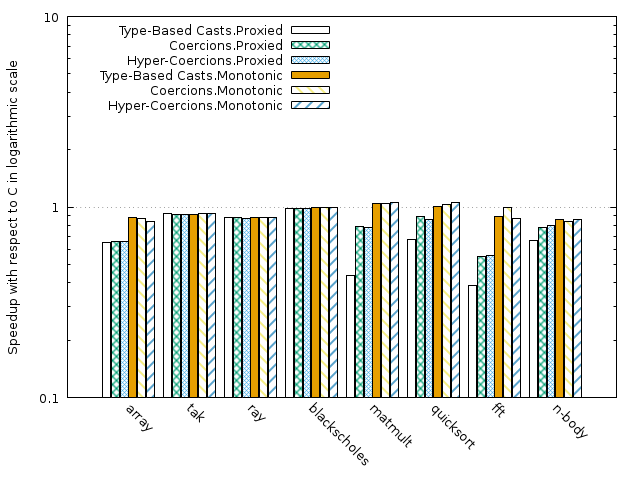
\includegraphics[scale=.47]{static.png}
  \caption{
    The logarithmic speedup of statically typed benchmarks
    with respect to C. Hyper-Coercions are shown as the light-blue
    striped (Proxied) and hatched (Monotonic) bars. The
    results indicated that there is little difference
    between coercions (green and yellow bars) and hyper-coercions. }
  \label{fig:static_results}
\end{figure}

\begin{figure}
  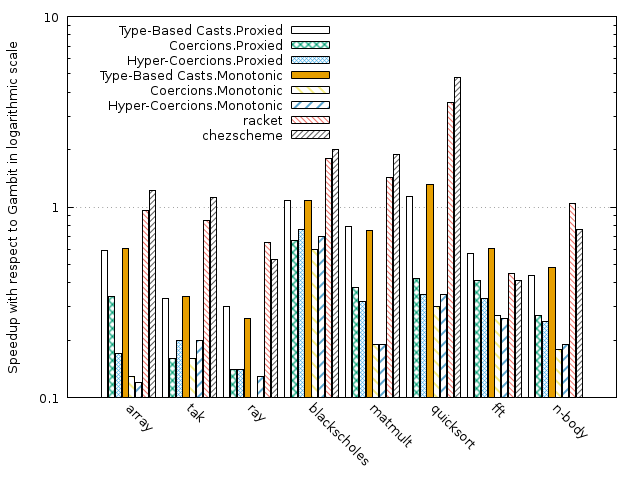
\includegraphics[scale=.47]{dyn.png}
  \caption{
    The logarithmic speedup of dynamically typed benchmarks
    with respect to gambit. Hyper-Coercions are show as the light-blue
    striped (Proxied) and hatched (Monotonic) bars. In general,
    the results for hyper-coercions track the performance of
    space-efficient coercions, but there is a large slowdown for
    hyper-coercions using proxies in the array benchmark.}
  \label{fig:dyn_results}
\end{figure}

\begin{figure}
  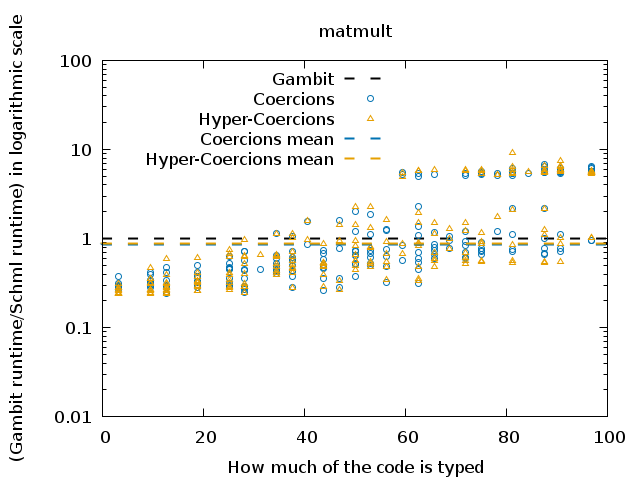
\includegraphics[scale=.45]{matmult_Proxied.png}
  \caption{The runtimes of the matrix multiplication benchmark
    with respect to Gambit while varying degree to which each
    program is statically typed.}
  \label{fig:grd_matmult}
\end{figure}

\begin{figure}
  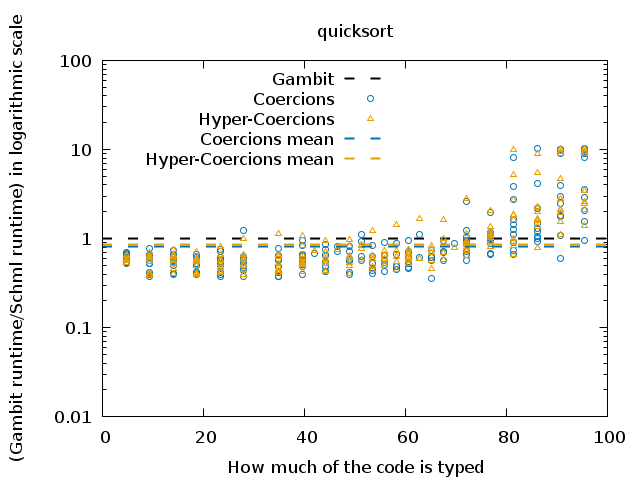
\includegraphics[scale=.5]{quicksort_Proxied.png}
  \caption{The runtimes of the quicksort benchmark with respect
    to Gambit while varying the degree to which each program
    is statically typed.}
  \label{fig:grd_quicksort}
\end{figure}

\paragraph{Why Hyper-Coercions Don't Improve Performance:}
We initially thought that the hyper-coercion representation
would improve performance, but careful reflection due to
these results indicates that we shouldn't have expected
significant gains from a naive implementation.
Most of this argument hinges on the fact that we suspect
that most common casts in a program are known statically.
This can obviously vary between programs, and we will
ultimately need empirical evidence to back this belief,
but if this is the case, then a naive implementation of
hyper-coercions is actually a slight deoptimization
over Schml's coercion representation. 

We suspected that the hyper-coercion representation
would primarily increase performance by decreasing
the amount of indirections through memory needed to
apply and compose coercions. This would indicate that
larger coercions with more indirections would benefit
more from the hyper-coercion representation than smaller,
less complex coercions. 
The casts that should benefit the most from hyper-coercions
are those that perform a projection, a mediating cast,
and an injection, and those that should benefit the
least are those that only perform a projection, intermediating
cast, or injection. In fact the current implementation
actually increases the number of indirections through
memory for lone intermediating casts. 

But if the most common casts are those that we know statically,
then the casts that benefit the least are actually the most
common case, because statically known casts never do more
than project, inject, or intermediate. Thus, one problem
with hyper-coercions are that they are optimizing for the uncommon case. 
This is made worse by the fact the Schml compiler optimizes
away the indirections for projections and injections for regular
coercions when they are not sub-components of intermediating coercions.
This means that, for projections and injections, the locality in
hyper-coercions should be equal and, for mediating coercions,
the locality has gotten worse. 

\section{Future Work}
\label{sec:future_work}
While the performance results of hyper-coercions are
disappointing, the Schml implementation of hyper-coercions
is very direct and doesn't optimize any cases where
hyper-coercions make it obvious that we should.
Many aspects of this could be cleared up without modifying
the semantics.

\paragraph{Compiling Static Coercions Better:}
We currently do not specialize the code that performs
casts where the input coercions are known. This is
something that we have considered,
but hyper-coercions make it obvious that we should,
because the casting operation for hyper-coercions
performs trivial but redundant work for all but
the most complicated coercions. The optimization
of cast code could be as simple as
hard coding the compiler for the most common
cases, but our compiler as a whole will benefit
most from a general purpose optimization pass
that runs after the lowering of casts.

\paragraph{Optimizing the most Common Cases:}
Hyper-Coercions that perform only an identity,
projection, injection, and intermediating cast
contain redundant information that isn't needed
for casting or composing. The most important case
to fix would be mediating coercions, because it
seems like this is the only place we are paying
for the hyper-coercion representation. This seems
like a fundamental flaw in hyper-coercions and
the model should be adjusted to help fix this
particular case. 

\paragraph{Characterizing Casts in Real Code}
The speculation that static known casts are most
common is just our intuition. We should investigate
the benchmarks that we currently support in order
to characterize the frequency and type of casts
that gradual programs generate. 

\paragraph{Increasing the Complexity of Benchmarked Code}
It could be the case that after these optimizations
the general trend is that hyper-coercions and coercions
still have equal performance. If this is the case we conjecture
that it is because none of the benchmarks use
complicated enough casts to benefit from hyper-coercions.
In this case we should investigate adding benchmarks that
that examine the highly gradual case that we believe hyper-coercions
should improve upon.

\bibliographystyle{abbrvnat}
\bibliography{all}

\end{document}
